\begin{center}
\begin{tikzpicture}[x=1cm,y=1cm]
%\pgfresetboundingbox
\draw[use as bounding box, anchor = north west,draw,dashed,gray] (-5.5,-3.25) rectangle (5.5,3.25);
\clip (-5.5,-3.25) rectangle (5.5,3.25);
%\node[anchor =north west] (text) at (-5.25,3.25){\begin{minipage}{10.0cm}
%\visible<1->{ We have built up the following picture:
%}
%\end{minipage}};
\visible<1->{\node (figure) at (0,0.75){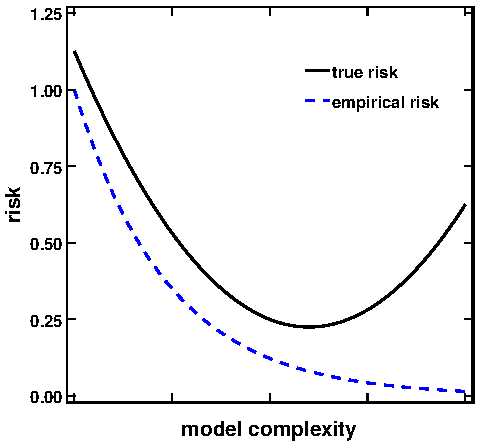
\includegraphics[width=5.25cm]{satistical_learning/figures/scheme_risk}};}
\visible<2->{\node[anchor =north west] (text) at (-5.25,-1.75){\begin{minipage}{10.0cm}
None of this helps us understand a how complicated our model should be.
\visible<3->{Unfortunately, \textbf{errors on our training data cannot tell us the answer}}
\end{minipage}};}
\end{tikzpicture}
\end{center}